\documentclass{article}
\usepackage[paper=a4paper, margin=1in]{geometry}
\usepackage{graphicx}
\usepackage{listings}
\usepackage{xcolor}
\usepackage[utf8]{inputenc}

\lstset{
  basicstyle=\ttfamily\small,
  breaklines=true,
  frame=single,
  language=C,
  keywordstyle=\color{blue},
  commentstyle=\color{green!50!black},
  stringstyle=\color{red}
}

\begin{document}

\title{Operating Systems Lab Assignment: Synchronization and Scheduling}
\author{Cameron Cleveland}
\date{October 24, 2025}
\maketitle

\section{Introduction}
This report documents the implementations and analyses for the synchronization and scheduling lab assignment, covering five provided problems and four additional exercises using mutexes and condition variables.

\section{Exercise 1: Hello World}
\lstinputlisting{hello_world.c}

\textbf{Explanation}:  
The original code had a race condition because the main thread could check or print before the child updated the shared flag. Adding a mutex and condition variable fixes this by letting the child safely update the flag while holding the lock, then signal the main thread. The main thread waits until the flag actually changes, so the output happens in the right order.

\textbf{Analysis}:  
This one really helped me see how condition variables work. They’re basically a clean way to “sleep” until something truly happens. The mutex keeps things atomic, so no one sees half-updated data. I also learned to always wait inside a loop with the lock, so I don’t miss signals or react to false ones.

\textbf{Screenshot}: Include a screenshot of compiling and running hello\_world.c.
\begin{figure}[h]
  \centering
  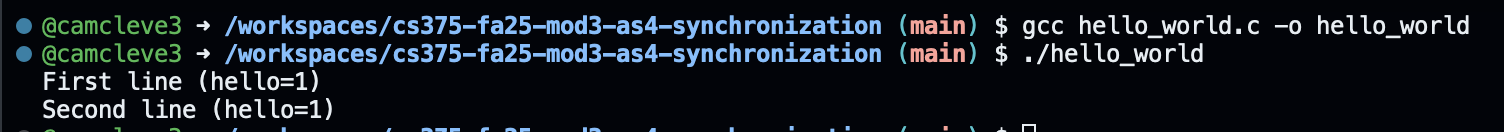
\includegraphics[width=\textwidth]{pic1.png}
  \caption{Compilation and execution of hello\_world.c}
\end{figure}

\section{Exercise 2: SpaceX Problems}
\lstinputlisting{spacex.c}

\textbf{Explanation}:  
The announcer thread ran too early because it wasn’t synced with the countdown. Using a mutex to protect the shared counter and a condition variable to make the announcer wait until it hits zero keeps everything in order. Once the countdown finishes, it signals the announcer to go.

\textbf{Analysis}:  
The main lesson here: only signal when the actual state changes, and always check that state under the mutex. Doing that guarantees the “launch” announcement happens right after the final countdown, never before.

\textbf{Screenshot}:
\begin{figure}[h]
  \centering
  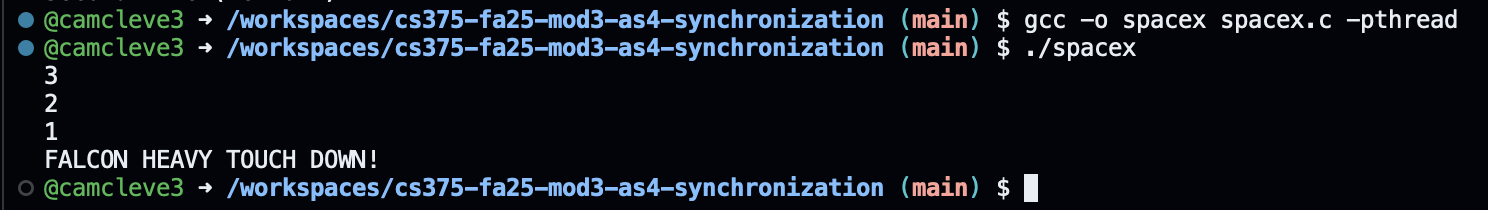
\includegraphics[width=\textwidth]{pic2.png}
  \caption{Compilation and execution of spacex.c}
\end{figure}

\section{Exercise 3: I Love You, Unconditionally!}
\lstinputlisting{love.c}

\textbf{Explanation}:  
The main thread needed to confirm that the helper thread really incremented the variable before printing the message. By locking, updating, and signaling from the helper, and having the main wait for that condition, we enforce a clean sequence.

\textbf{Analysis}:  
This showed me how Mesa-style condition variables actually behave. A signal doesn’t mean “it’s true now,” it means “go check again.” You always recheck the condition under the mutex to avoid race conditions and misleading wakeups.

\textbf{Screenshot}:
\begin{figure}[h]
  \centering
  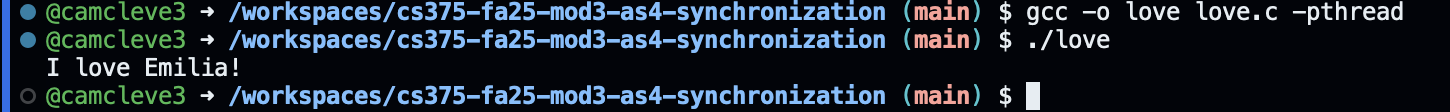
\includegraphics[width=\textwidth]{pic3.png}
  \caption{Compilation and execution of love.c}
\end{figure}

\section{Exercise 4: Locking Up the Floopies}
\lstinputlisting{floppy.c}

\textbf{Explanation}:  
The deadlock came from inconsistent lock ordering: two threads could each grab one account lock and freeze waiting for the other. Fixing that means deciding on a global order, like by account ID, and always locking in that sequence.

\textbf{Analysis}:  
It’s a simple rule but it makes all the difference. Consistent lock order removes cycles in the resource graph, which removes deadlocks. After that, all transfers can run at once without freezing the program.

\textbf{Screenshot}:
\begin{figure}[h]
  \centering
  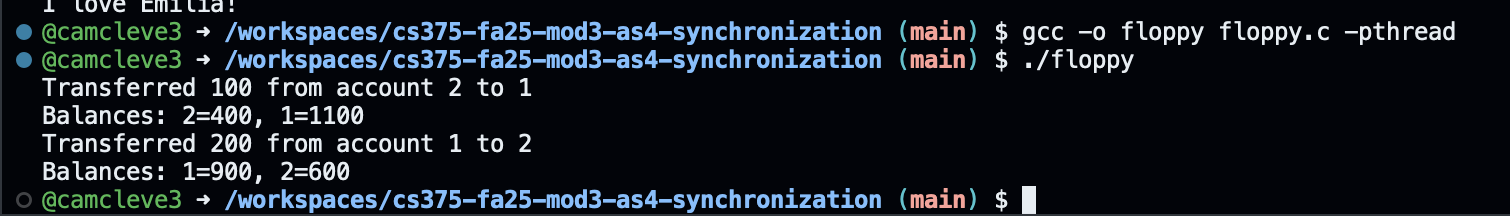
\includegraphics[width=\textwidth]{pic4.png}
  \caption{Compilation and execution of floopy.c}
\end{figure}

\section{Exercise 5: Baking with Condition Variables}
\lstinputlisting{baking.c}

\textbf{Explanation}:  
There were multiple threads for ingredients, heating, and eating, all needing coordination. Condition variables let each thread wait for the right bowl state: ingredients wait for space, the heater waits for the mix to be ready, and the eater waits until baking is done.

\textbf{Analysis}:  
This exercise made me think of synchronization as choreography, each step depending on the last one finishing. The mutex protects shared state, and condition variables control timing. Waiting in loops keeps everyone in sync even if timing shifts slightly.

\textbf{Screenshot}:
\begin{figure}[h]
  \centering
  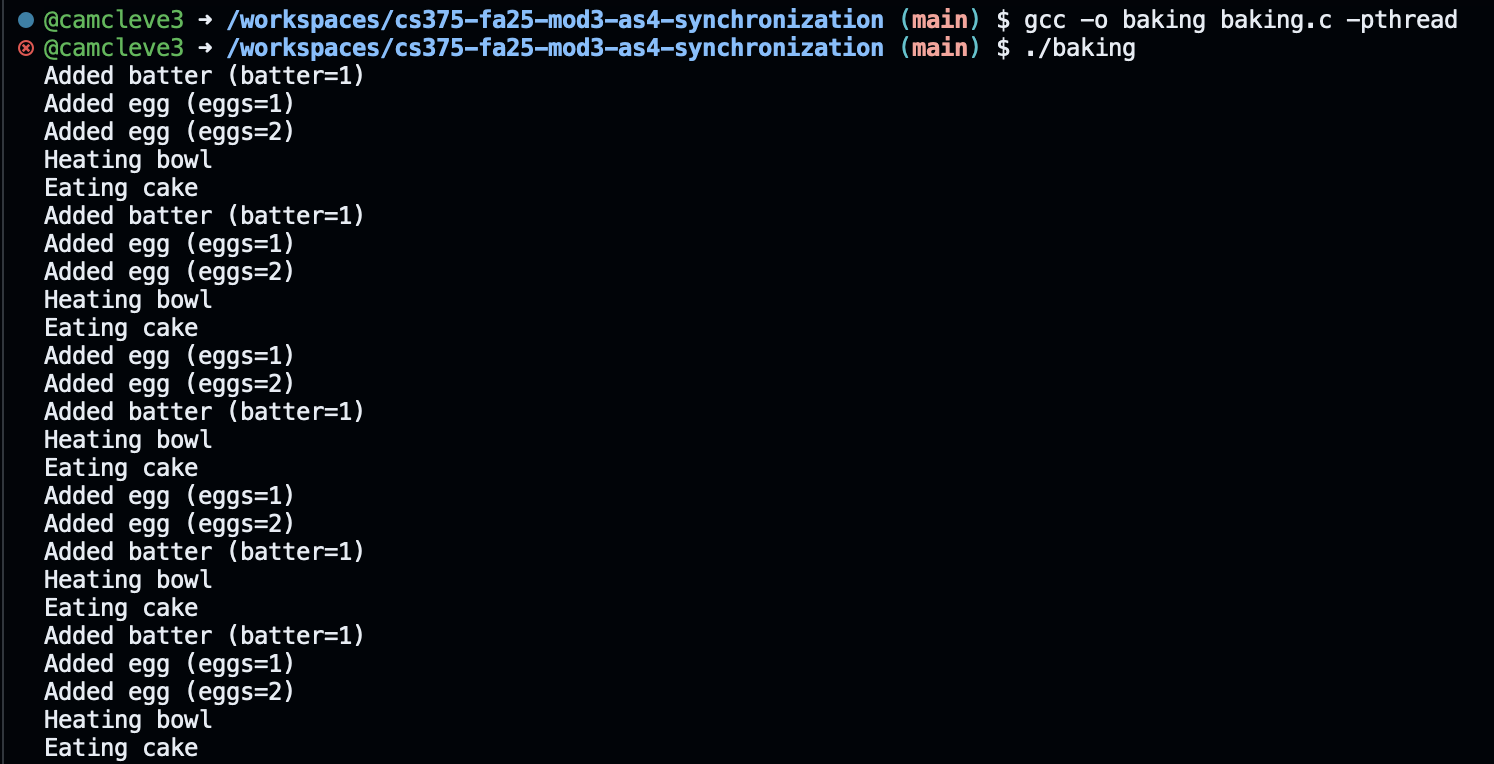
\includegraphics[width=\textwidth]{pic5.png}
  \caption{Compilation and execution of baking.c}
\end{figure}

\section{Exercise 6: Priority Donation in Transfer}
\lstinputlisting{priority_transfer.c}

\textbf{Explanation}:  
Priority inversion happens when a low-priority thread holds a lock that a high-priority thread needs. Priority donation fixes that by temporarily boosting the lock-holder’s priority until it finishes the critical section, then lowering it back.

\textbf{Analysis}:  
This made me appreciate how scheduling and synchronization overlap. Donation prevents high-priority threads from getting stuck behind slower ones, which keeps the system fair and responsive.

\textbf{Screenshot}:
\begin{figure}[h]
  \centering
  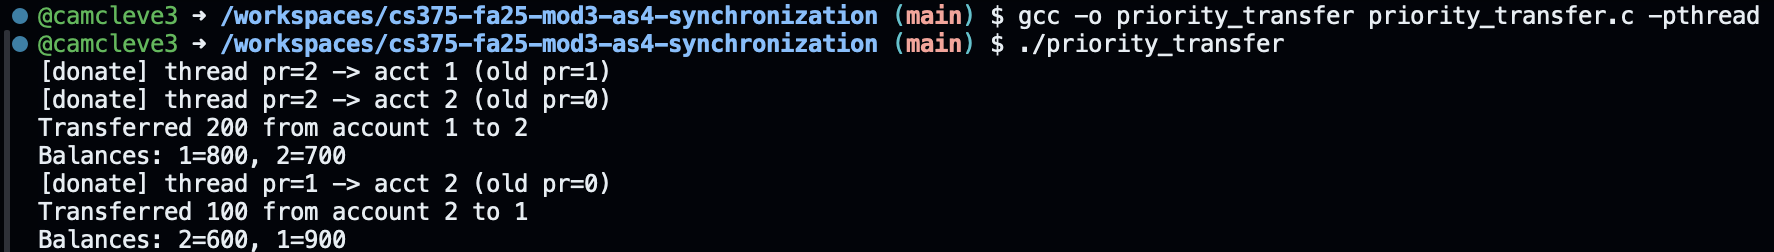
\includegraphics[width=\textwidth]{pic6.png}
  \caption{Compilation and execution of priority\_transfer.c}
\end{figure}

\section{Exercise 7: Barrier Synchronization}
\lstinputlisting{barrier.c}

\textbf{Explanation}:  
A barrier makes all threads pause until everyone reaches the same point, then they all continue together. It uses a mutex, an arrival counter, and a generation variable so it can be reused safely for multiple rounds.

\textbf{Analysis}:  
The generation check is the real trick. It ensures that no thread runs ahead. Every “Before” happens before any “After,” which keeps the output clean and the barrier reusable.

\textbf{Screenshot}:
\begin{figure}[h]
  \centering
  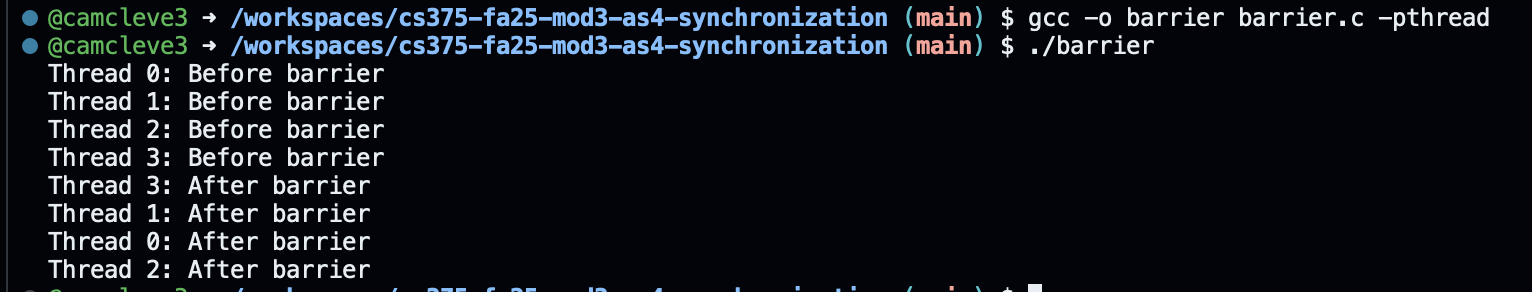
\includegraphics[width=\textwidth]{pic7.png}
  \caption{Compilation and execution of barrier.c}
\end{figure}

\section{Exercise 8: Readers-Writers with Priority}
\lstinputlisting{readers_writers.c}

\textbf{Explanation}:  
Writer priority means if a writer wants access, readers should hold off until the writer is done. The fix blocks new readers while a writer is waiting or active, lets current readers finish, and then wakes the writer.

\textbf{Analysis}:  
It’s a balancing act: give writers priority without starving readers. The mutex guards the shared counters, and condition variables manage entry. It showed me how fair scheduling can be built directly into synchronization logic.

\textbf{Screenshot}:
\begin{figure}[h]
  \centering
  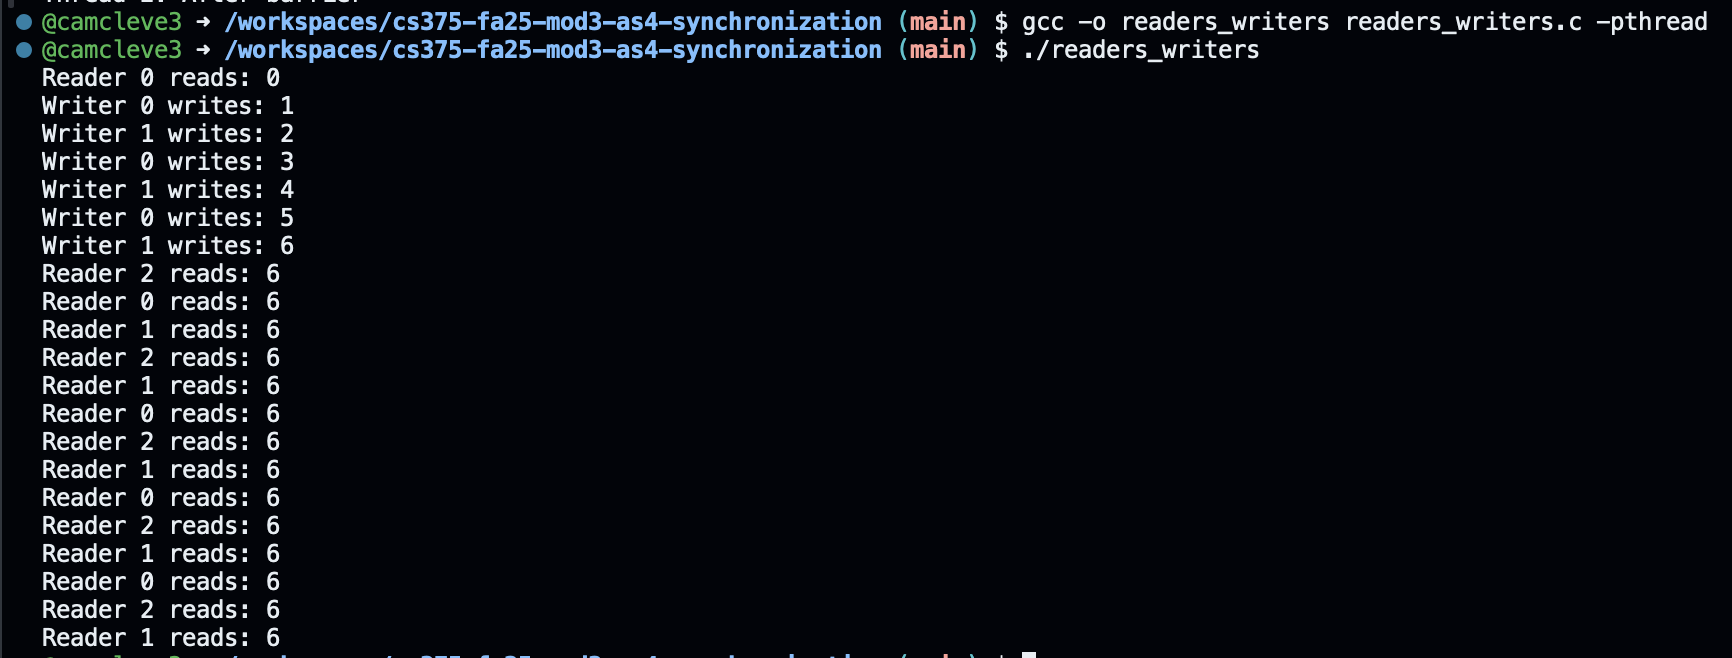
\includegraphics[width=\textwidth]{pic8.png}
  \caption{Compilation and execution of readers\_writers.c}
\end{figure}

\section{Exercise 9: Thread Pool}
\lstinputlisting{thread_pool.c}

\textbf{Explanation}:  
The thread pool keeps a fixed set of worker threads pulling jobs from a shared queue. The queue uses mutexes and condition variables so producers wait if it’s full and workers sleep if it’s empty.

\textbf{Analysis}:  
This design saves a ton of overhead since threads are reused instead of constantly created and destroyed. The synchronization keeps everything safe and efficient, no spinning or wasted CPU time.

\textbf{Screenshot}:
\begin{figure}[h]
  \centering
  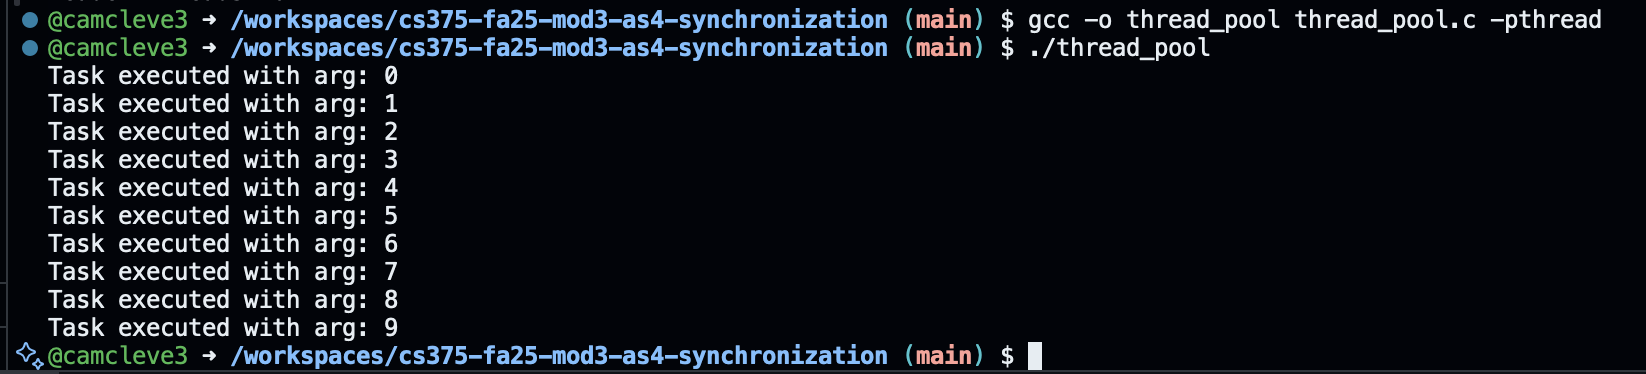
\includegraphics[width=\textwidth]{pic9.png}
  \caption{Compilation and execution of thread\_pool.c}
\end{figure}

\end{document}
